%------------------------------------------------------------------------------
%	PACKAGES AND THEMES
%------------------------------------------------------------------------------

\documentclass[aspectratio=169,xcolor=dvipsnames,handout]{beamer}
\usetheme{Darmstadt}
\usecolortheme{seahorse}
\usepackage[hangul]{kotex}
\usepackage{hyperref}
\usepackage{amsfonts, amssymb}
\usepackage{graphicx} 
\usepackage{array, booktabs, multicol, multirow} % Allows the use of \toprule, \midrule and \bottomrule in tables
\setbeamercovered{transparent}

%------------------------------------------------------------------------------
%	MY COMMAND
%------------------------------------------------------------------------------

\newcommand{\R}{\mathbb{R}}
\newcommand{\y}{\mathbf{y}}

%------------------------------------------------------------------------------
%	TITLE PAGE
%------------------------------------------------------------------------------

\title[분배정의철학]{분배정의철학} 
\subtitle{경제정의와 불평등}
\author[오성재]{오성재}
\institute[HNU] % Your institution as it will appear on the bottom of every slide, may be shorthand to save space
{%
    한남대학교 \\
    탈메이지 교양학부 \\
}
\date{\today} 

%------------------------------------------------------------------------------
%	PRESENTATION SLIDES
%------------------------------------------------------------------------------

\begin{document}

\begin{frame}
    \titlepage
\end{frame}

\begin{frame}{목차}
    \tableofcontents
\end{frame}

\section{들어가는 말}

\begin{frame}[<+->]
\frametitle{분배적 정의의 범위}
    \begin{itemize}
        \item 분배적 정의는 사람들이 원하는 것이 그 사람들에게 어떻게 나눠져 있는가에 관심. 
        \begin{exampleblock}{}
        \begin{itemize}
            \item 전국민 재난지원금.
            \item 수자원의 올바른 사용처(콘서트 vs. 농지).
        \end{itemize}
        \end{exampleblock}
        \item 일반적인 법$\cdot$사회영역의 정의와 관심대상이 다름.
        \begin{exampleblock}{}
        \begin{itemize}
            \item 특정사안(간통, 대마초)에 합법화.
            \item 범죄자에 대한 적정형량.
        \end{itemize}
        \end{exampleblock}
    \end{itemize}
\end{frame}

\begin{frame}[<+->]
\frametitle{기회비용}
    \begin{itemize}
        \item 일상생활에서 주로 사용하는 비용은 회계적 비용이다.
        \item 반면, 경제학에서 고려하는 모든 비용은 \textbf{기회비용}이다.
        \begin{block}{기회비용}
            어떤 선택으로 인해 포기된 기회들 가운데 가장 큰 가치를 갖는 기회 자체 또는 그러한 기회가 갖는 가치를 말한다.
        \end{block}
        \begin{exampleblock}{대학진학의 비용}
        대학진학의 비용은 다음과 같다.
        \begin{itemize}
            \item 회계비용 : 대학등록금 + 생활비.
            \item 기회비용 : 대학등록금 + 4년간의 수입.
        \end{itemize}
        \end{exampleblock}
    \end{itemize}
\end{frame}

\section{분배적 정의에 대한 이론들}
\begin{frame}[<+->]
    \begin{itemize}
       \item (분배적)정의에 관한 여러 입장을 나누는 첫번째 기준은 권리(the right)와 선(the good)에 대한 입장에서 시작.
       \item 목적론 : 선이 권리보다 우선한다.
        \begin{itemize}
           \item 정의는 사람들이 진정으로 선을 달성할 수 있도록 허용하는 일련의 규칙.
        \end{itemize}
       \item 의무론 : 권리가 좋은 것에 우선한다.
        \begin{itemize}
           \item 정의는 우리의 다양한 목적을 허용 가능하게 추구할 수 있는 방법을 알려주고 또한 우리가 추구할 수 있는 목적을 제한한다.
        \end{itemize}
    \end{itemize}
\end{frame}
   
\begin{frame}[<+->]
\frametitle{목적론}
    \begin{itemize}
        \item 무엇이 사람들이 사회속에서 살아가는데 좋게 만드는 가에 관심.
        \begin{exampleblock}{선의 예시}
        \begin{itemize}
            \item (개인과 재산의) 안전; 공동체; 
            \item 안정성 및 (제도, 관계, 재화와 용역의 공급에 대한) 예측가능성;
            \item 학습, 교육; 문화 및 과학;
            \item 보건, 주거; 기술 및 기타 좋은 생활의 수단.
        \end{itemize}
        \end{exampleblock}
        \item 정의는 우리가 원하는 것, 또는 우리가 진정으로 원해야 하는 것을 가장 잘 얻을 수 있게 해주는 규칙.
    \end{itemize}
\end{frame}

\begin{frame}[<+->]
\frametitle{목적론 : 완벽주의 vs. 공리주의}
    \begin{itemize}
        \item  목적론적 정의 이론은 목적을 객관적 선으로 보는지 주관적인 선으로 보는지에 따라 두 가지로 나눔.
        \item \textbf{완벽주의} : 정의로운 사회는 우리가 객관적으로 좋은 인간의 삶을 살 수 있도록 하는 사회.
        \begin{itemize}
            \item 완벽주의 안에서도 객관적 선에 대한 서로 다른 생각이 분파를 낳음.
            \item 완벽주의는 역사적으로 지배적인 정의론 이었으나, 현대에는 객관적으로 좋은 삶이라는 개념이 사람에 따라 다르다는 점에서 소수의 시각으로 좁혀짐.
        \end{itemize}
        \item \textbf{공리주의} : 사람들이 (자신이 원하는 것을 얻는다는 의미에서) 주관적으로 좋은 삶을 사는 것이 중요.
        \begin{itemize}
        \item 사회는 사람들이 원하는 상품을 함께 생산하는 일종의 협동조합.
        \item 정의란 자신이 원하는 것을 많이 가지게 하는 것.
        \end{itemize}
    \end{itemize}
\end{frame}

\begin{frame}[<+->]
\frametitle{의무론 : 계약론 vs. 권리론}
    \begin{itemize}
        \item 정의는  사회의 목적에 그 자체가 아니라, 목적을 추구하는 방법에 관심을 가져야.
        \item \textbf{계약론} : 사회적 번영을 위한 협력적 추구가 모든 협력자에게 공정한 방식으로 수행되어야 함.
        \begin{itemize}
            \item 사회를 구성하는 것이 바람직한 결과의 생산과 분배를 위한 전제 조건이고, 모든 구성원이 협력하므로 재화의 분배는 사회의 모든 구성원에게 공정해야.
        \end{itemize}
        \item \textbf{권리론} : 정의의 주제는 행동이며 한 사람의 행동이 다른 사람의 권리와 어떻게 관련되는지에 관심.
        \begin{itemize}
            \item 정의로운 사회는 단순히 권리(자연적이든 후천적이든)가 존중되는 사회.
            \item 정의가 자연적 권리와 획득한 권리를 보호하고 존중하는 것이라면, 생산되는 총체적 상품이나 이러한 상품이 어떻게 분배되는지에 초점을 맞추는 것은 잘못.
        \end{itemize}
    \end{itemize}
\end{frame}

\section{분배적 정의의 원칙들}
\begin{frame}[<+->]
\frametitle{분배적 정의의 원칙}
    \begin{itemize}
        \item 평등(equalit)의 원칙
        \item 충분성(sufficiency)의 원칙
        \item 우선(proority)의 원칙
        \item 효용(utility)의 원칙
        \item 공로(merit)의 원칙
        \item 자유(liberty)의 원칙
    \end{itemize}
\end{frame}

\begin{frame}[<+->]
\frametitle{평등의 원칙}
    \begin{itemize}
        \item 불평등은 그 자체로 정의롭지 않다. 따라서 평등 분배는 어떤 불평등 분배보다 정의롭다.
        \item 평등분배를 위해서 타인을 끌어내리는 것 역시 정당화 할 수 있다.
    \end{itemize}
    \begin{alertblock}{평등지상주의?}
    \begin{itemize}
        \item 맹인 한 사람이 존재하는 사회가 평등주의를 달성하려면?
        \item 능력이나 노력에 관계없이 모두가 동등한 결과를 얻는 사회는 정의로운가?
    \end{itemize}
    \end{alertblock}
\end{frame}

\begin{frame}[<+->]
\frametitle{충분성의 원칙}
    \begin{itemize}
        \item 모두가 충분하게 가지는 것이 중요하다.
        \item 소유의 상대적 비교(격차의 유무, 크기)는 중요하지 않다.
    \end{itemize}
    \begin{alertblock}{빈곤의 판단}
    \begin{itemize}
        \item 상대적 빈곤 : 중위소득자의 50\%.
        \item 절대적 빈곤 : 일일 소득 5,000원.
    \end{itemize}
    \end{alertblock}
\end{frame}

\begin{frame}[<+->]
\frametitle{우선의 원칙}
    \begin{itemize}
        \item 분배에서 가장 열악한 위치에 처한 사람들이 개선되어야 한다.
    \end{itemize}
    \begin{figure}
        \centering
        \caption{간단한 소득분포}
        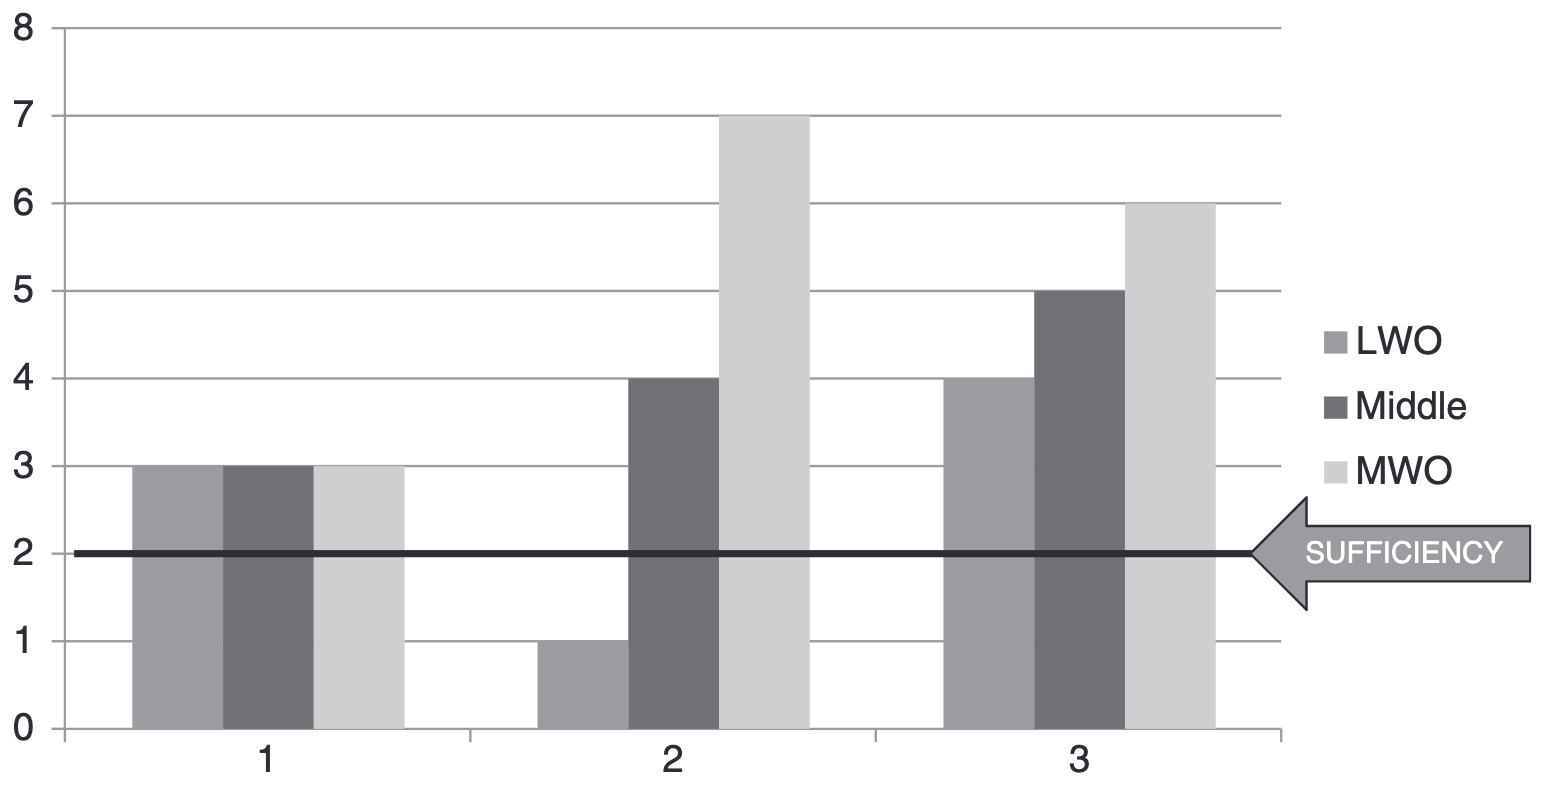
\includegraphics[width=.5\textwidth]{pic/fig1_2.png}
    \end{figure}
\end{frame}

\begin{frame}[<+->]
\frametitle{효용의 원칙}
    \begin{itemize}
        \item 순효용(이익과 손해의 차이)을 극대화 하는 분배가 정당한 분배이다.
        \item 불평등이나 빈곤의 증가는 순효용의 극대화를 위한다면 가능하다.
    \end{itemize}
    \begin{figure}
        \centering
        \caption{분배정의 원칙에 맞는 소득분포}
        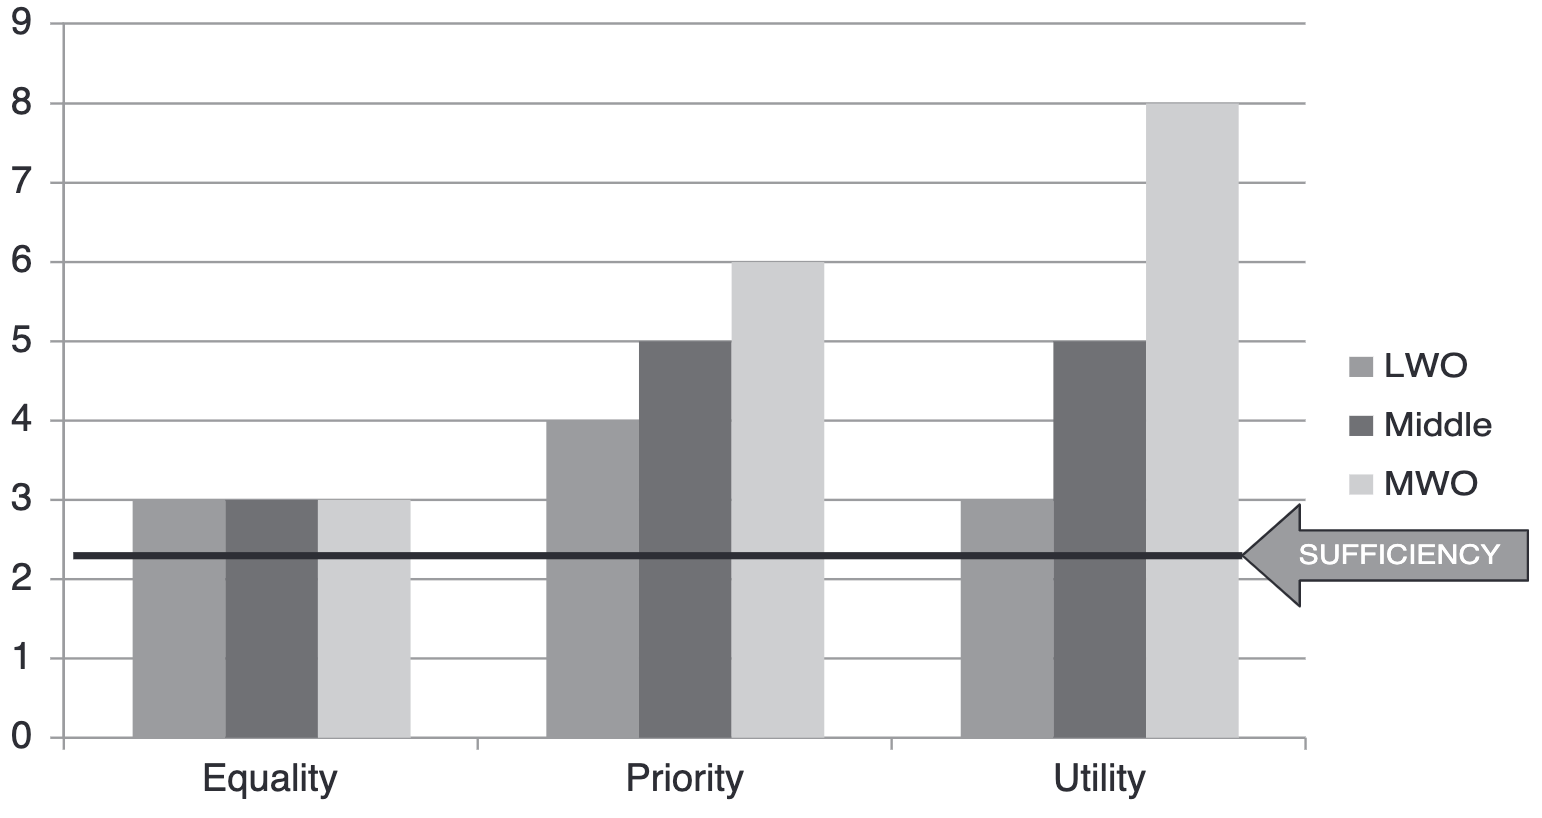
\includegraphics[width=.5\textwidth]{pic/fig1_4.png}
    \end{figure}
\end{frame}

\begin{frame}[<+->]
\frametitle{공로의 원칙}
    \begin{itemize}
        \item 개인의 공로나 자격(desert)을 반영한 분배가 정당하다.
        \item 자격으로서의 공로 : 가장 자격있는 자가 얻는다.
        \item 노력으로서의 공로 : 기여한 만큼 얻는다.
        \item 동일한 기여를 하면 같은 몫을 얻을 수 있다는 점에서 형평(equity)의 원칙으로도 볼 수 있음.
    \end{itemize}
\end{frame}

\begin{frame}[<+->]
\frametitle{자유의 원칙}
    \begin{itemize}
        \item 정당한 분배는 사람들의 소유의 형태로 판단할 수 없다.
        \item 개인들 간에 모든 자발적 행위의 결과는 정당하다.
        \item 분배의 역사적 과정이 중요하다.
        \item 순수한 절차적 정의.
    \end{itemize}
\end{frame}

\end{document}
